\chapter{Methodology}\label{sec:method}
In this section, we first define the problem and present some preliminaries. Then we discuss our proposed model in detail and the connection between our model and the other existing works.

\begin{table}[t]
	% \renewcommand{\arraystretch}{1}
	\centering
	\caption{Notations and descriptions}\label{tab:notation}
	\resizebox{\columnwidth}{!}{
		\begin{tabular}{c|l}
			\hline
			Notation & Description. \\
			\hline
			$u, v$ & The target user and the target item. \\
			$M, N$ & The number of users and items. \\
			$y, \hat{y}$ & The indicator and the predicted probability of the user-item interaction. \\
			$\bm{u}, \bm{v}$ & Dense representation of target user $u$ and target item $v$.\\
			$\mg_t^k(u), \mg_t^k(v)$ & K-hop \textit{user/item-rooted interaction set} at time slice $t$.\\
			$\mg_t(u), \mg_t(v)$ & \textit{user/item-rooted interaction set} at time slice $t$.\\
			$\mg^t(\cdot)$ & The incremental graph at the $t$-th time slice.\\
			% $\bm{E}_{\mg_t^k(u)}, \bm{E}_{\mg_t^k(v)}$ & Dense representations of items/users in $\mg_t^k(u)$ and $\mg_t^k(v)$.\\
			% $e$ & Dense representation of user (or item) in $\mg_t^k(u)$ (or $\mg_t^k(v)$).\\
			$\bm{u}_t^{k}, \bm{v}_t^{k}$ & Aggregated user/item-side representation of k hop(s) graph information \\
			& at time slice $t$.\\
			$U, V$ & User/item-side sequence.\\
			$\Delta T$ & Time interval to split subgraphs.\\
			$S$ & Size of \textit{user/item-rooted interaction set}.\\
			\hline
		\end{tabular}
	}
\end{table}

\begin{figure*}[t]
	\centering
	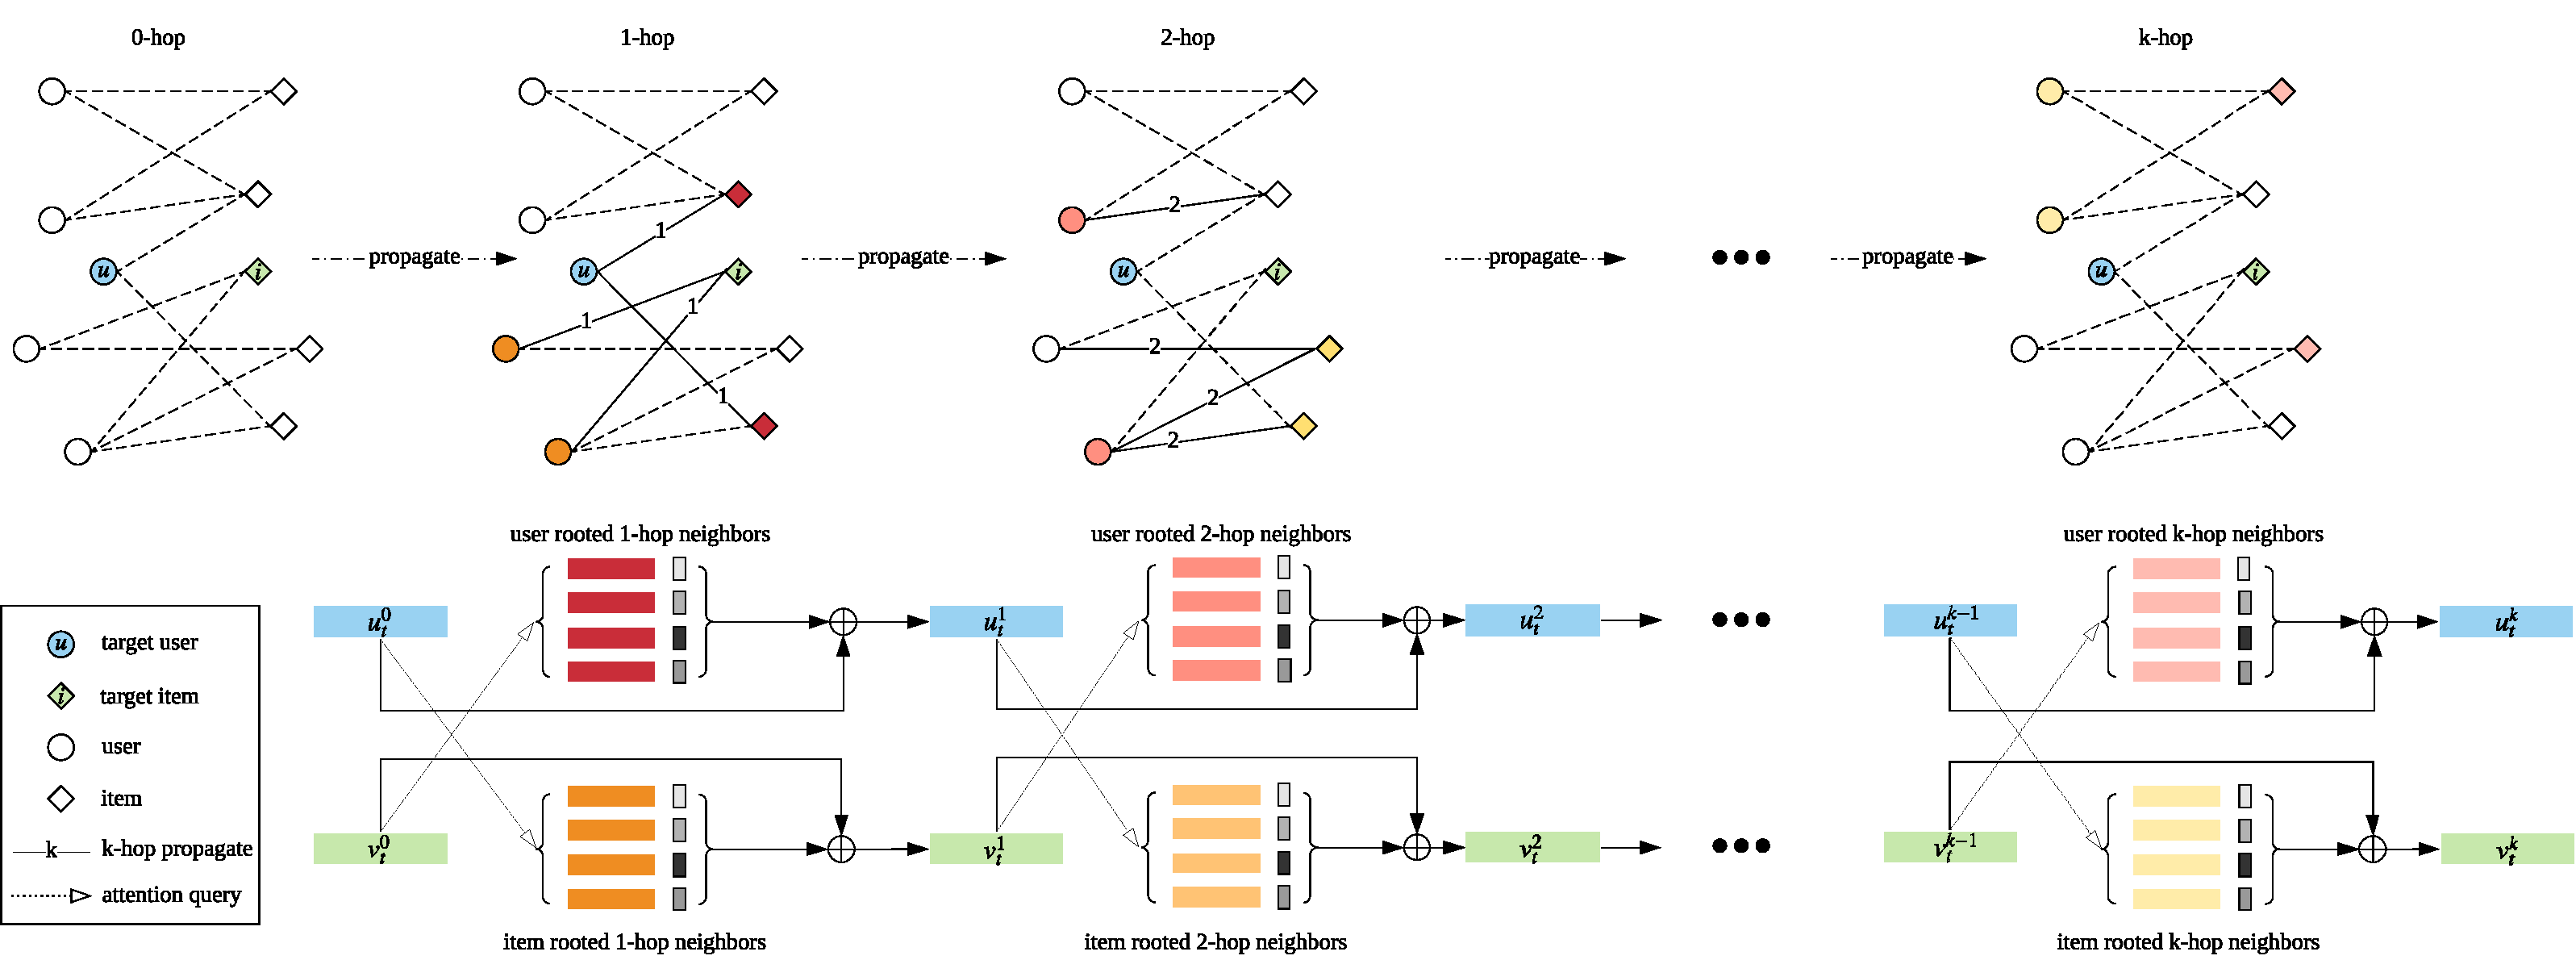
\includegraphics[width=1.0\textwidth]{score_spatial.pdf}
	\caption{Multi-hop Co-Attention Graph Network calculation process.}
	\label{fig:spatial-framework}
	\vspace{-10pt}
\end{figure*}

\section{Preliminaries}\label{sec:preliminaries}
In a recommender system, there are $M$ users in $\mathcal{U}=\{u_1, \ldots, u_M\}$ and $N$ items in $\mathcal{V}=\{v_1, \ldots, v_N\}$.
We regard the user-item interactions as a bipartite graph $\mg$ whose nodes are users and items while its edges are interactions defined as
% In the history, any user may reveal interests on some items and the interaction behaviors would be tracked in the system as $\mathcal{Y}=\{y_{uv} | u \in \mathcal{U}, v \in \mathcal{V} \}$ and
\begin{equation}
	y_{ij} = \left\{
		\begin{array}{rcl}
			1, & & i~(\text{user}/\text{item})~ \text{has interacted with} ~j~(\text{item}/\text{user}); \\
			0, & & \text{otherwise.} \\
		\end{array}
	\right.
\end{equation}
The user-item interaction $y$ is either implicit feedback \cite{agarwal2009spatio}, i.e., clicks or explicit user rating \cite{koren2009collaborative}.
Without loss of generality, we focus on the implicit feedback which is more common in practice\cite{zhou2018deepa,ren2019lifelong,guo2017deepfm}.

\subsection{User/Item-Rooted Interaction Set}
From a start node on the graph, we could take multiple hops, and gather a series of nodes which are the neighbors of the start node with different distance. 

Hereby we define \textit{user-rooted interaction set} of the target user $u$ at distance $k$ hops as
\begin{equation}
\mg^k(u) = \{j|y_{ij}=1, i \in \mg^{k-1}(u) \}
\end{equation}
and $\mg^{0}(u) = \{u\}$ which contains only the root node. Symmetrically, we define \textit{item-rooted interaction set} of the target item $v$ as 
\begin{equation}
\mg^k(v) = \{j|y_{ij}=1, i \in \mg^{k-1}(v) \}
\end{equation}
and $\mg^{0}(v) = \{v\}$.

There is some collaborative information retrieved through this propagation process. As for the view of user, the k-hop \textit{user-rooted interaction set} $\mg^k(u)$ contains item nodes ($k=2n-1, n \in N^{+}$) and user nodes when $k = 2n, n \in N^{+}$. The items in $\mg^k(u)$ and $\mg^{k+2}(u)$ both attract the same group of users that are in $\mg^{k+1}(u)$, while the users in $\mg^{k+1}(u)$ and $\mg^{k+3}(u)$ demonstrate similar interests on the items in $\mg^{k+2}(u)$. 
These collaborative patterns are useful for the subsequent modeling.
%These relations that users share same intersts and items show similar attractions are the \textbf{collaborative} information that we may use for the subsequent modeling.
And the situation of the target item is symmetrically similar. 

We combine all the information obtained through $K$-hop propagation to form the \textit{user-rooted interaction set} and \textit{item-rooted interaction set} as $\mg(u) = \bigcup_{k=0}^K \mg^k(u)$ and $\mg(v)=\bigcup_{k=0}^K \mg^k(v)$.
% \subsection{Interaction Set}
% % graph
% Given the target user $u$, we can conduct the \textit{interaction set} of user $u$ as
% \begin{equation}
% \mg(u) = \{v_i | y_{uv_i}=1 \}.
% \end{equation}
% The user's interaction set is the collection of all the items that the user has interacted with.
% From the view of the user-rooted interaction graph, we may regard $\mg_u$ as the 1-hop neighboring nodes from the root node $u$, as is illustrated in Figure~\ref{fig:bi-graph}.

% It is natural to expand the user-rooted interaction graph and find the \textit{co-interaction set} as
% \begin{equation}
% 	\mg(v|u) = \{ u_j | y_{{u_j}{v_i}}=1, v_i \in \mg_u \}.
% \end{equation}
% The co-interaction set includes all the users who have also interacted with the items in $\mg(u)$, i.e., they may share the similar tastes with the user $u$.
% From the view of graph, all the users in $\mg(v|u)$ are represented as the nodes through 2-hop from the root user $u$.
% Here we only care about the interaction and co-interaction sets of $u$ and we have omitted the other interaction connections through multi-hop ($>2$) relations from the root user, since it may bring more noise than useful patterns. In many works of GNN, using 2-hop neighbors is good enough.\jiarui{citation of GNN work}

% The above disscussion is from the user side, while we may also define the interaction set $\mg(v)$ and the co-interaction set $\mg(u|v)$ of the given item $v$ from the item side with similar definition.
% The differences lie in the meaning of the ``interaction'' where, from the item side, the items in the co-interaction set $\mg(u|v)$ share the similar properties to the given item $v$ for they have interactions with same group of users.

\subsection{Evolving Interaction Graph}
Now that we have defined the local interaction graph $\mg$ of the user $u$ and the item $v$, we take one step forward and consider the incremental evolving interaction graphs along the time to capture temporal dynamics of both user and item.
%For example, during a specific time period, the users may make several interactions with some items; 
Specifically, the users (items) may conduct different interactions with other items (users) at different time.
Thus, the whole interaction graph is evolving all the time and consisted of several incremental subgraphs.

To better model the dynamic temporal patterns of the interaction graphs, we slice the whole graph to $T$ sliced subgraphs, each of which is constructed within a unified time interval. So that
\begin{equation}
\begin{aligned}
	\mg(\cdot) &= \bigcup_{t=1}^T \mg_t(\cdot), \\
\end{aligned}
\end{equation}
where $\mg_t(\cdot)$ contains all the interactions happened during the $t$-th time slice.
Specifically, the \textit{user-rooted interaction set} at $t$-th time slice is denoted as $\mg_t(u)$ and the \textit {item-rooted interaction set} is $\mg_t(v)$

\subsection{Task Definition}
The goal of the recommender system is to estimate the probability of interactions $\hat{y}$ between the target user $u \in \mathcal{U}$ and the given item $v \in \mathcal{V}$, with consideration of the user-rooted subgraph $\mg_u$ and the item-rooted subgraph $\mg_v$ as
\begin{equation}
\hat{y}_{uv} = \mathit{f}(u, v| \mg_u, \mg_v; \btheta)
\end{equation}
through the learned function $\mathit{f}$ with parameters $\btheta$ where $\mg_u = \bigcup_{t=1}^T \mg_t(u)$ and $\mg_v=\bigcup_{t=1}^T \mg_t(v)$.
We conclude the notations and the corresponding description in Table~\ref{tab:notation}.



\section{Spatial Graph Pattern Mining}\label{sec:spatial}
In this section, we describe the proposed \textit{Co-Attention Graph Network} for handling the user/item-rooted subgraphs. We also present an importance sampling strategy used to retrieve more related neighbors while avoiding noise.


\subsection{Co-Attention Graph Network}
At each time slice $t$, we use \textit{Co-Attention Graph Network} to aggregate subgraph information. We take the view of the target user $u$ as an example.
The propagated information of different user (or item) nodes in $\mg^k_t(u)$ would contribute differently to the final recommendation decisions.
Traditional method like GAT \cite{velivckovic2017graph} and \cite{song2019session} utilize the spatial information of the local graph through calculating attentional relatedness between the center node and its nearest neighboring nodes, which has no relevance to the target item and may be unsuitable for recommender system.
%Take $\mg^1_t(u)$ as an example, the items in $\mg^1_t(u)$ should be weighted by the target item $v$ instead of their center node $u$. And it is not suitable when we consider the multi-hop senario. \jiarui{how to express that this bottom-up way is not suitable for recommendation domain?}

To address this problem, we propose \textit{Co-Attention Graph Network}. As illustrated in~Fig \ref{fig:spatial-framework}, for the k-th hop propagation, we calculate user-side representation and item-side representation as
\begin{equation}
\bm{u}_t^k = \bm{u}_t^{k-1} + \sum_i \alpha_{ui}^k e_i^k ~,
\end{equation}
\begin{equation}
\bm{v}_t^k = \bm{v}_t^{k-1} + \sum_i \alpha_{vi}^k e_i^k ~,
\end{equation}
where $e_i^k$ is the $d$-dimensional dense embedding of users (or items) in the k-hop \textit{user/item-rooted interaction set}. And We set $\bm{u}_t^0 = \bm{u}$, $\bm{v}_t^0 = \bm{v}$. The co-attention weights $\alpha_{ui}^k$ and $\alpha_{vi}^k$ are calculated as

\begin{equation} \label{eq:co_atten_1}
\alpha_{ui} = \frac{exp(LeakyReLU(\bm{a^T}[\bm{We}_i^k||\bm{Wv_t^{k-1}}]))}{\sum_{\bm{e}_j^k \in \mg^k(u)}exp(LeakyReLU(\bm{a^T}[\bm{We}_j^k||\bm{Wv_t^{k-1}}]))}
\end{equation}

\begin{equation}  \label{eq:co_atten_2}
\alpha_{vi} = \frac{exp(LeakyReLU(\bm{a^T}[\bm{We}_i^k||\bm{Wu_t^{k-1}}]))}{\sum_{\bm{e}_j^k \in \mg^k(v)}exp(LeakyReLU(\bm{a^T}[\bm{We}_j^k||\bm{Wu_t^{k-1}}]))}
\end{equation}
Here $\bm{W} \in R^{d \times d}$ is weight matrix of a shared linear transformation which applied to every node's representation. $||$ is a concatenate operation, $\bm{a} \in R^{2d \times 1}$ is the weight vector of a single-layer feedforward neural network with LeakyReLU activation function which is
\begin{equation}
%y_{ij} = \left\{
%\begin{array}{rcl}
%1, & & i~(\text{user}/\text{item})~ \text{has interacted with} ~j~(\text{item}/\text{user}); \\
%0, & & \text{otherwise.} \\
%\end{array}
%\right.
	LeakyReLU(x) = \left\{
		\begin{array}{ccr}
		x, x \geq 0; \\
		\frac{x}{\gamma}, x < 0,
		\end{array}
	\right.
\end{equation}
where negative input slop $\gamma = 0.2$. Then it is normalized by softmax function.

Please note that we use an iterative way to aggregate multi-hop information. The target item's representation $\bm{v}_t^{k-1}$ from the last iteration, i.e., $(k - 1)$-hop, is used as a query to calculate the co-attention weight values of the $k$-th hop neighbors of the target user $u$. 
$\bm{v}_t^{k-1}$ contains not only the target item's own information, but the collaborative information of its neighbors from all the previous $(k - 1)$ hops.
And we make symmetrically the similar operation for the target item.
%the target item's side uses user representation as attention query. 
In this way, the representations of both the target user and the target item are correlated and collaborative. This collaborative view from both sides to do graph learning is proved an effective way in the experiments in Section~\ref{sec:ab-study}.

% \subsubsection{Co-Attention Mechanism for 2-hop Neighbors}
% In this section, we describe the co-attention mechanism that is used to utilize 2-hop spatial information. We need to find collaborative relations between two groups of nodes: one group is the users in $\mg(v)$ and $\mg(v|u)$, the other is the items in $\mg(u)$ and $\mg(u|v)$, as is illustrated in Figure~\ref{fig:framework}.

% Take $\mg(u)$ and $\mg(v|u)$ as an example, $\bm{E}_{\mg(u)} \in R^{K_1 \times d}$ and $\bm{E}_{\mg(v|u)} \in R^{K_2 \times d}$ are embedding matrix of $\mg(u)$ and $\mg(v|u)$ respectively. The affinity matrix $\bm{C} \in R^{K_1 \times K_2}$ is calculated as 
% \begin{equation}
% 	\bm{C} = F_p(\bm{E}_{\mg(u)}) \bm{A} (F_q(\bm{E}_{\mg(v|u)}))^T
% \end{equation}
% where $F_p(\cdot)$ and $F_q(\cdot)$ are one-layer neural network functions with ReLU activation function for $\bm{E}_{\mg(u)}$ and $\bm{E}_{\mg(v|u)}$ respectively and $\bm{A} \in R^{d \times d}$ is an attentive matrix.

% After calculating the affinity matrix $\bm{C}$, we conduct max-pooling (MP) operation along rows of $\bm{C}$ respectively to generate importance vector $\bm{a}^{col} \in R^{K_2 \times 1}$ for $\bm{E}_{\mg(v|u)}$, and the importance vector is then normalized by softmax function.
% \begin{equation}
% 	\bm{a}_j^{col'} = MP(\{\bm{C}_{ij}\}_{i=1}^{K_1})%\bm{a}_i^{row'} = MP(\{\bm{C}_{ij}\}_{j=1}^{K_2}),~~~
% \end{equation}
% \begin{equation}
% 	\bm{a}^{col} = Softmax(\bm{a}^{col'})%\bm{a}^{row} = Softmax(\bm{a}^{row'}),~~~
% \end{equation}
% So, the aggregated representation of user-side 2-hop neighbors is
% \begin{equation}
% 	\bm{u}^{(2)}_t = \sum_{j \in [0, K_2-1]} \bm{a}_j^{col} * \bm{E}_{\mg(v|u)}^j
% \end{equation}
% where $\bm{E}_{\mg(v|u)}^j$ is the j-th row of the embedding matrix.

% In a symmetric way, we can get the item-side 2-hop neighbors representation $\bm{v}^{(2)}_t$.
% % explain the meaning of the co-attention calculation
% By using the co-attention mechanism, we give the relevant 2-hop neighbors more attention than those that are not very relevant so that the noise introduced by the 2-hop expansion can be reduced.
% In this way, we effectively utilize the 2-hop spatial information and find relations between user rooted subgraph and item rooted subgraph at each time slice.

\subsection{Importance Sampling Strategy with Local Graph Structure}\label{sec:sampling}
When we do the $k$-th propagation from $\mg_t^{k-1}(u)$ (or $\mg_t^{k-1}(v)$), there could be a lot of nodes in $\mg_t^k(u)$ and it could introduce too much noise. Thus we need an importance sampling strategy for each propagation process.
% which will sample the most relative nodes in the next hop.
When doing sampling, we could regard the \textit{user/item-rooted subgraph} as a directed graph, the direction is the propagation direction from $(k-1)$-th hop to $k$-th hop, as the propagation from $\mg^{k-1}_t(u)$ to $\mg^k_t(u)$ which is illustrated in Fig.~\ref{fig:sampling}.

We calculate the importance factor of node $p$ in $\mg^k_t(u)$ as
\begin{equation}
	\bm{I}_p = \sum_{q \in pre(p)} \frac{1}{\textit{out-degree}(q)}
\end{equation}
where $pre(p)$ contains the predecessor nodes of node $p$ (which is $\mg^{k-1}_t(u)$ in Fig.~\ref{fig:sampling}).
Then the importance factors are normalized by a softmax function and used as sampling probabilities as 
\begin{equation}
	\bm{Pr}_p = \frac{\exp(\bm{I}_p)}{\sum_{n\in \mg^{k}_t(u)} \exp(\bm{I_n})} ~.
\end{equation}

If a node in $\mg^k_t(u)$ has more predecessors, it indicates that the node is more important and more related to the previous nodes. However, if the predecessor is very popular (out-degree is large), then the relatedness from this predecessor is reduced. 
The reason to punish the predecessor nodes with their popularity is the following: when we consider the nodes in $\mg^{k-2}_t(u)$ which are the same type to the nodes in $\mg^k_t(u)$ (both are users or items), relation though a very popular intermedia node (in $\mg^{k-1}_t
(u)$) is not that important than a relation though a not popular intermedia node. In this way, we could find more similar and related collaborative nodes in $\mg^{k}_t(u)$.
%\kan{needs refine.}


\begin{figure}[h]
	\centering
	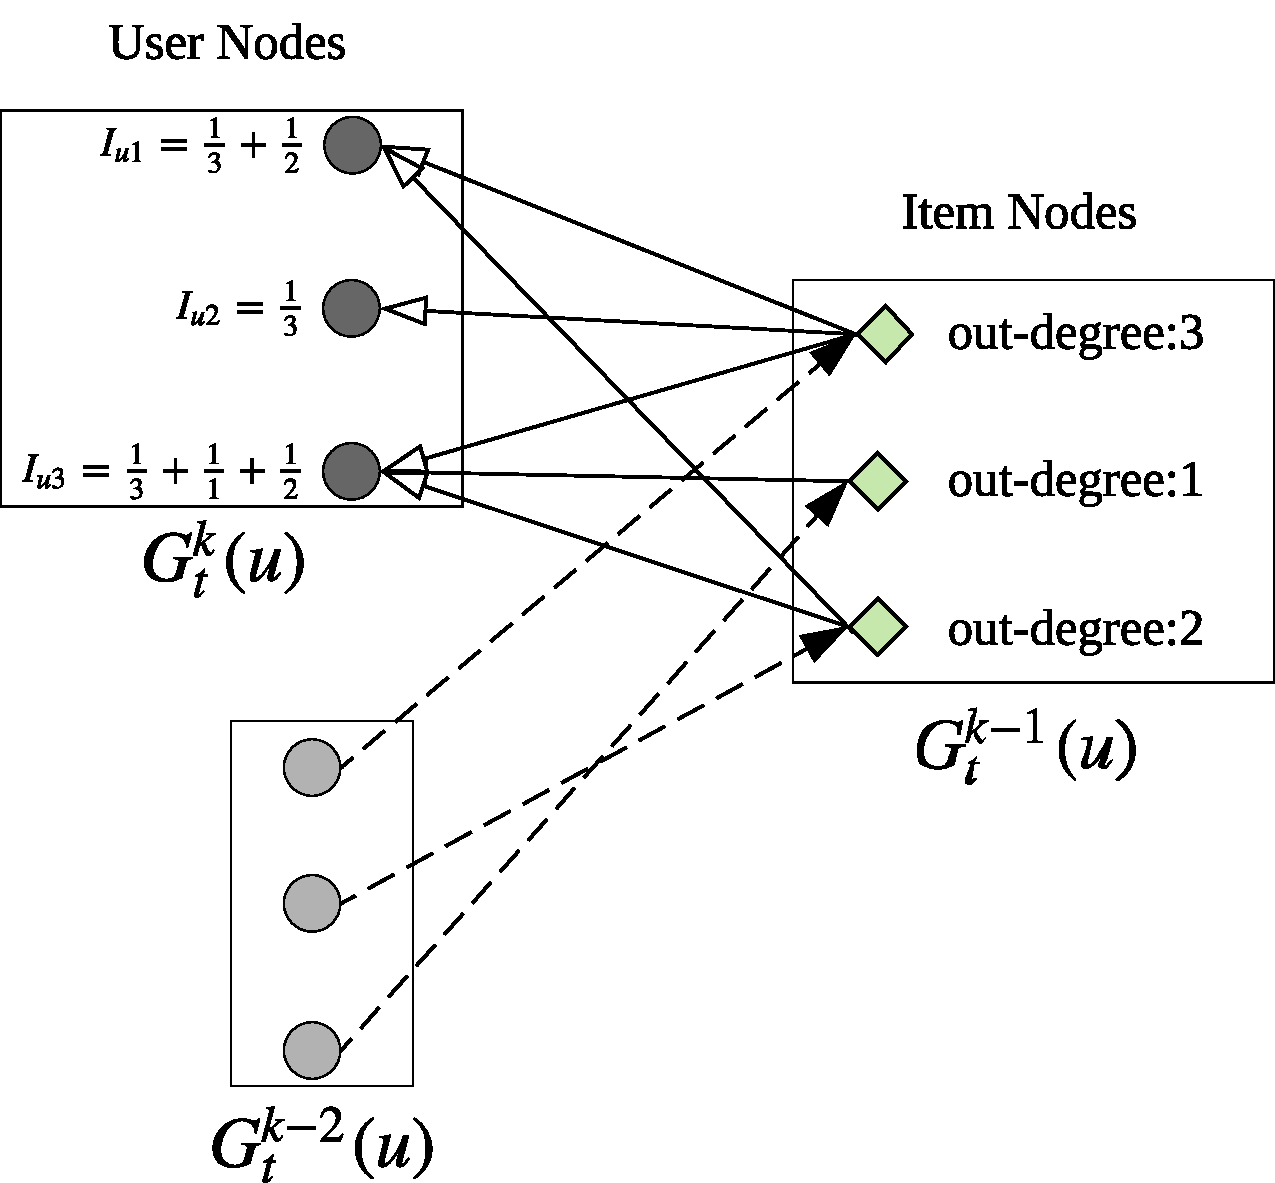
\includegraphics[width=0.7\columnwidth]{importance_sampling.pdf}
	\caption{Illustration of importance sampling of $\mg_t^k(u)$.}
	\label{fig:sampling}
	\vspace{-10pt}
\end{figure}
% \subsubsection{Co-Attention Mechanism}\label{sec:co-atten}
% We first formulate and present co-attention mechanism that we use in our model\cite{hu2018local}. $\bm{P} \in R^{m \times d}$ and $\bm{Q} \in R^{n \times d}$ are the two sets which need to be jointly represented. The affinity matrix $\bm{C} \in R^{m \times n}$ is calculated as
% \begin{equation}
% 	\bm{C} = F_p(\bm{P}) \bm{A} (F_q(\bm{Q}))^T
% \end{equation}
% where $F_p(\cdot)$ and $F_q(\cdot)$ are multi-layer neural network functions for $\bm{P}$ and $\bm{Q}$ respectively and $\bm{A} \in R^{d \times d}$ is an attentive matrix.

% After calculating the affinity matrix $\bm{C}$, we conduct max-pooling (MP) operation along rows and columns of $\bm{C}$ respectively to generate importance vectors for $\bm{P}$ and $\bm{Q}$.
% \begin{equation}
% 	\bm{a}_i^p = MP(\{\bm{C}_{ij}\}_{j=1}^n),~~~\bm{a}_j^q = MP(\{\bm{C}_{ij}\}_{i=1}^m)
% \end{equation}
% Then we conduct softmax function on both $\bm{a}^p$ and $\bm{a}^q$ and get normalized importance vectors.
% Finally, we use the normalized importance vectors to perform weighted sum on $\bm{P}$ and $\bm{Q}$ and get final representations as
% \begin{equation}
% 	\bm{p} = \bm{P}^T \bm{a}^p, ~~~\bm{q} = \bm{Q}^T \bm{a}^q
% \end{equation}
% \subsubsection{Use of Co-Attention}
% Co-attention mechanism is used to mining spatial relations and aggregate the graph information within one time slice. We use embedding mechanism to map each item and user to a low-dimensional space, so user-side 1-hop sub graph $\mg^t(u)$ and item-side 2-hops sub graph $\mg^t(v|u)$ are mapped to relative embedding matrices. And the embedding matrices are used as the $\bm{P}$ and $\bm{Q}$ in \ref{sec:co-atten} relatively and the two sub graphs are represented as $\bm{u}_t^{(1)}$ and $\bm{v}_t^{(2)}$. Similarly, $\mg^t(v)$ and $\mg^t(u|v)$ are treated in the same way, so we get $\bm{v}_t^{(1)}$ and $\bm{u}_t^{(2)}$ relatively.


\section{Temporal Interactive Dual Sequence Modeling} \label{sec:temporal}
As the sequential recommendation task can be regarded as a dynamic graph link prediction problem described in Section~\ref{sec:preliminaries}, in this section, we describe the method we use to model the temporal incremental graphs and the proposed \textit{Interactive Attention} used for dual sequence modeling.

\subsection{Temporal Dynamics of Incremental Graphs}
For each time slice, we get the representations of target user $u$ and target item $v$ as $\bm u_t^K$ and $\bm v_t^K$, respectively. These representations are the results after $K$ hops propagation and aggregation which is described in Section~\ref{sec:spatial}.
After that we get two sequences $U$ and $V$, which are the sequences of target user's and item's multi-hop representation respectively. For simplicity, we denote $\bm u_t = \bm u_t^K$ and $\bm v_t = \bm v_t^K$ and
\begin{equation}
U = \{\bm{u}_1, \bm{u}_2, ..., \bm{u}_{T}\}~,
V = \{\bm{v}_1, \bm{v}_2, ..., \bm{v}_{T}\} .
\end{equation}

We use Gated Recurrent Unit \cite{cho2014learning} (GRU) to model the temporal dynamics for  target user-side and target item-side. Each GRU model takes the corresponding graph representation $\bm u_t^K$ at each time step and the hidden state $\bh_{t-1}$ from the last time step, and then calculates as
\begin{equation}\small
\begin{aligned}
\bm{z}_t^u =& ~\sigma (\overline{\bm{W}}_z^u \bm{u}_t + \overline{\bm{U}}_z \bh_{t-1}^u + \overline{\bm{b}}_z^u) \\
\bm{r}_t^u =& ~\sigma (\overline{\bm{W}}_r^u \bm{u}_t + \overline{\bm{U}}_r \bh_{t-1}^u + \overline{\bm{b}}_r^u) \\
\bh_{t}^u =& ~(1 - \bm{z}_t^u) \odot \bh_{t-1}^u  \\
&~~~~~~~~~~~~~~~~~+ \bm{z}_t^u \odot \tanh(\overline{\bm{W}}_h^u \bm{u}_t + \overline{\bm{U}}_h^u (\bm{r}_t^u \odot \bh_{t-1}^u) + \overline{\bm{b}}_h^u)  ~,
\end{aligned}
\label{eq:gru}
\end{equation}
where $\odot$ is the element-wise product operator. 

The item-side temporal dynamics are modeled in the same way. Till now, we've got user-side and item-side sequence of temporal nodes representations: $\{\bm h_1^u, \bm h_2^u, ..., \bm h_T^u\}$ and $\{\bm h_1^v, \bm h_2^v, ..., \bm h_T^v\}$.

\subsection{Interactive Attention Mechanism of Dual Sequence} \label{sec:attention}
As illustrated in Fig~\ref{fig:temporal-framework}, different time slice has different impact on the final prediction at $T + 1$. And hereby we introduce our \textit{Interactive Attention Mechanism}. Unlike the attention mechanism in \cite{zhou2018deepb} and \cite{zhou2018deepa} which uses target item to query the interacted items sequence, we utilize dual sequences information at the same time interactively to weigh across different time slice.
The attention value of each time slice $\beta_t$ is calculated as,
\begin{equation}
relation_t = \sigma(\bm Q_2(\sigma(\bm Q_1((\bm h_t^u \odot \bm h_t^v) || (\bm u \odot \bm v)))))
\end{equation}

\begin{equation}
\beta_t = \frac{\exp(relation_t)}{\sum_{i=1}^T \exp(relation_i)}
\end{equation}
where $\sigma$ is ReLU activation function and $\bm Q_1$, $\bm Q_2$ are weight matrix of the two-layer MLP.

And the final representations of target user and target item are 
\begin{equation} \label{eq:seq_rep}
\bm r_u = \sum_{t=1}^T \beta_t \bm h_t^u, ~~~~\bm r_v = \sum_{t=1}^T \beta_t \bm h_t^v
\end{equation}

In this way, we utilize dual sequences information to calculate attention weights which reflect interaction intensity of each time slice. Different from common attention mechanism used in sequential recommendation/user response prediction task \cite{zhou2018deepb, zhou2018deepa} which uses target item as query and retrieve the most relevant user historical behaviors, we model the relations between target user and item at each time slice interactively from both sequences and give them different importance. The effectiveness of the proposed \textit{Interactive Attention} is shown in Section.~\ref{sec:ab-study}.

\begin{figure}[t]
	\centering
	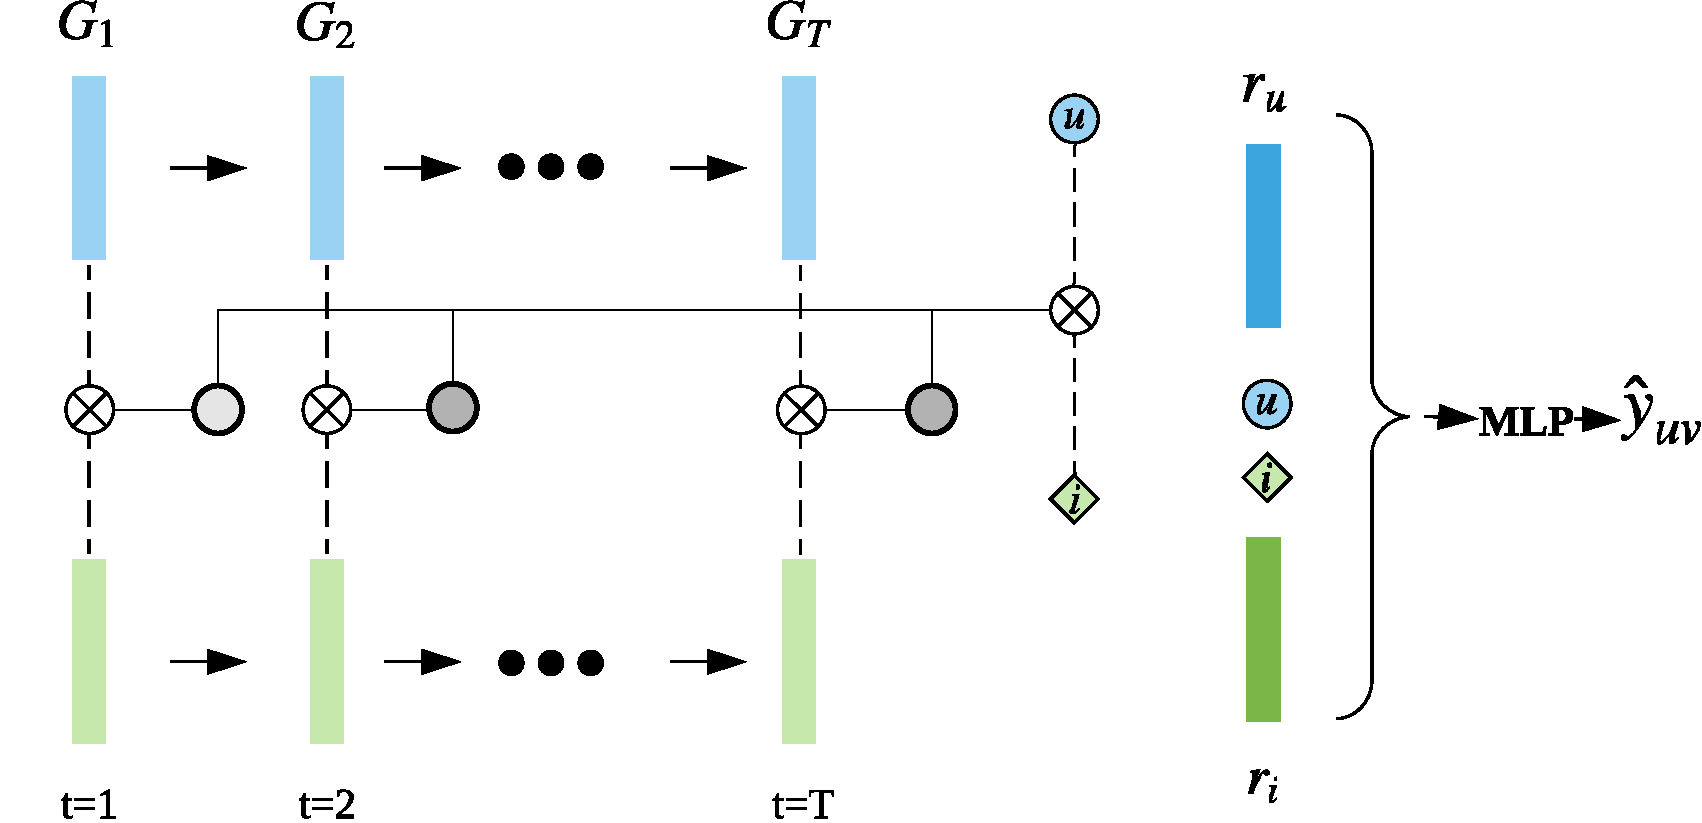
\includegraphics[width=1.0\columnwidth]{score_temporal.pdf}
	\caption{Temporal Interactive Dual Sequence Modeling of SCoRe.}
	\label{fig:temporal-framework}
	\vspace{-10pt}
\end{figure}


\section{Final Prediction and Loss Functions}
The predicted probability of interaction between the target user and the target item is calculated as
\begin{equation}
\hat{y} = f(\bm{r}_u, \bm{r}_v, \bm{u}, \bm{v}; \bm{\Theta}),
\end{equation}
where $f$ is implemented as a multi-layer perceptron with the ReLU activation function. The parameters set of the MLP is $\bm{\Theta}$.
The inference procedure is illustrated in Figure~\ref{fig:temporal-framework}.

As for the loss function, we take an end-to-end training and introduce (i) the widely used cross entropy loss $\mathcal{L}_{\text{ce}}$ \cite{ren2018bid,zhou2018deepa,zhou2018deepb} over the whole training dataset with (ii) the parameter regularization $\mathcal{L}_{\text{r}}$. We utilize stochastic gradient descent for optimization. Thus the final loss function is
\begin{equation}
\begin{aligned}
\argmin_{\bm{\Theta}, \bm{\Phi}} &= \mathcal{L}_{\text{ce}} + \lambda \mathcal{L}_r \\
&= -\sum_{s} \big[ y_s \log \hat{y}_s + (1-y_s) \log (1-\hat{y}_s)\big] \\
& + \frac{1}{2} \lambda \left( \|\bm{\Theta} \|_2^2 + \| \bm{\Phi} \|_2^2 \right) ~,
\end{aligned}
\end{equation}
where $\bm{\Phi}$ includes the parameters in GRUs, $\bm{W}$, $\bm{a}$ in \textit{Co-Attention Graph Network} and $\bm Q_1$, $\bm Q_2$ of \textit{Interactive Attention Mechanism}.

\section{Relations to Previous Works}
The proposed model can be simplified to previous frameworks of recommender systems:

\begin{itemize}[leftmargin=15pt]
	\item \textbf{Dual Sequence Framework:} If we only use 1-hop neighbors of the target user and the target item, as $u_t = u_t^1$ and $v_t = v_t^1$, and treat each neighbor and each time slice equally, \score~ would have the same structure as RRN \cite{wu2017recurrent} and GCMC \cite{fadel2018link}.
	\item \textbf{Single Sequence Framework:} If we eliminate the item-side sequence from the dual sequence framework above and make each time slice only has one interaction, we might get the framework of sequential recommendation models similar to RNN models \cite{hidasi2015session,ren2019lifelong,zhou2018deepb}.
	\item \textbf{Non Sequence Framework:} If we don't consider the temporal dynamics of user interests of the above single sequence framework, and consider the user behaviors as a whole, then \score~ might degenerate to the traditional CF models \cite{koren2008factorization}.
\end{itemize}